% Part: model-theory
% Chapter: interpolation
% Section: separation

\documentclass[../../../include/open-logic-section]{subfiles}

\begin{document}

\olfileid{mod}{int}{sep}

\olsection{Separation of \printtoken{P}{sentence}}

A bit of groundwork is needed before we can proceed with the proof of
the interpolation theorem. An interpolant for $!A$ and $!B$ is
!!a{sentence}~$!C$ such that $!A \Entails !C$ and $!C \Entails !B$.
By contraposition, the latter is true iff $\lnot !B \Entails \lnot
!C$. !!^a{sentence}~$!C$ with this property is said to \emph{separate}
$!A$ and $\lnot !B$.  So finding an interpolant for $!A$ and $!B$
amounts to finding !!a{sentence} that separates $!A$ and $\lnot !B$.
As so often, it will be useful to consider a generalization: a
sentence that separates two \emph{sets} of !!{sentence}s.

\begin{defn}
A sentence $!C$ \emph{separates} sets of sentences $\Gamma$ and
$\Delta$ if and only if $\Gamma \Entails !C$ and $\Delta \Entails
\lnot !C$. If no such !!{sentence} exists, then $\Gamma$ and $\Delta$
are \emph{inseparable}.
\end{defn}

The inclusion relations between the classes of
models of $\Gamma$, $\Delta$ and $!C$ are represented below:
\begin{figure}[h]
  \ollabel{fig:sep}
  \centering
  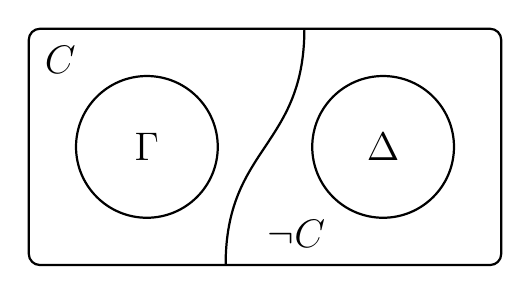
\begin{tikzpicture}[node distance=2cm, auto, thick]
    \draw [rounded corners] (0,0) -- (6,0) -- (6,3) -- (0,3) --  cycle;
    \draw (1.5,1.5) circle (0.9cm);
    \draw (4.5,1.5) circle (0.9cm);
    \path node at (1.5,1.5) {\Large $\Gamma$}; 
    \path node at (4.5,1.5) {\Large $\Delta$}; 
    \path node at (0.4,2.6) {\Large $\formula{C}$};
    \path node at (3.4,0.4) {\Large $\lnot \formula{C}$};
    \draw (2.5,0) .. controls (2.5,1.5) and (3.5,1.5) .. (3.5,3);
  \end{tikzpicture}
  \caption{$!C$ separates $\Gamma$ and $\Delta$}
\end{figure}


\begin{lem}\ollabel{lem:sep1}
Suppose $\Lang{L}_0$ is the language containing every !!{constant},
!!{function} and !!{predicate} (other than $\doteq$) that occurs in
\emph{both} $\Gamma$ and $\Delta$, and let $\Lang{L}'_0$ be obtained
by the addition of infinitely many new !!{constant}s $\Obj c_n$ for $n
\ge 0$. Then if $\Gamma$ and $\Delta$ are inseparable in $\Lang{L}_0$,
they are also inseparable in $\Lang{L}'_0$.
\end{lem}

\begin{proof}
We proceed indirectly: suppose by way of contradiction that $\Gamma$
and $\Delta$ are separated in $\Lang{L}'_0$. Then $\Gamma \Entails
\Subst{!C}{c}{x}$ and $\Delta \Entails \lnot \Subst{!C}{c}{x}$ for some $!C \in
\Lang{L}_0$ (where $c$ is a new !!{constant}---the case where $!C$
contains more than one such new !!{constant} is similar). By
compactness, there are \emph{finite} subsets $\Gamma_0$ of $\Gamma$
and $\Delta_0$ of $\Delta$ such that $\Gamma_0 \Entails \Subst{!C}{c}{x}$
and $\Delta_0 \Entails \lnot \Subst{!C}{c}{x}$. Let $!G$ be the
conjunction of all !!{formula}s in $\Gamma_0$ and $!H$ the
conjunction of all !!{formula}s in $\Delta_0$. Then
\begin{align*}
  !G & \Entails \Subst{!C}{c}{x}, & !H  \Entails \lnot \Subst{!C}{c}{x}.
\end{align*}
From the former, by Generalization, we have $!G \Entails
\lforall[x][!C]$, and from the latter by contraposition,
$\Subst{!C}{c}{x} \Entails \lnot !H$, whence also $\lforall[x][!C]
\Entails \lnot \delta$. Contraposition again gives $!H \Entails
\lnot \lforall[x][!C]$. By monotony,
\begin{align*}
  \Gamma &\Entails \lforall[x][!C], & 
  \Delta & \Entails \lnot \lforall[x][!C],
\end{align*}
so that $\lforall[x][!C]$ separates $\Gamma$ and $\Delta$ in
$\Lang{L}_0$. 
\end{proof}

\begin{lem}\ollabel{lem:sep2}
Suppose that $\Gamma \cup \{ \lexists[x][!S] \}$ and $\Delta$ are
inseparable, and $c$ is a new !!{constant} not in $\Gamma$, $\Delta$,
or $!S$. Then $\Gamma \cup \{ \lexists[x][!S], \Subst{!S}{c}{x} \}$
and $\Delta$ are also inseparable.
\end{lem}

\begin{proof}
Suppose for contradiction that $!C$ separates $\Gamma \cup \{
\lexists[x][!S], \Subst{!S}{c}{x}\}$ and $\Delta$, while at the same
time $\Gamma \cup \{\lexists[x]{!S} \}$ and $\Delta$ are
inseparable. We distinguish two cases:
\begin{enumerate}
\item $c$ does not occur in $!C$: in this case $\Gamma \cup
  \{\lexists[x][!S], \lnot!C \}$ is satisfiable (otherwise $!C$
  separates $\Gamma \cup \{\lexists[x][!S] \}$ and $\Delta$). It
  remains so if $\Subst{!S}{c}{x}$ is added, so $!C$ does not separate
  $\Gamma \cup \{ \lexists[x][!S], \Subst{!S}{c}{x} \}$ and $\Delta$
  after all.
\item $c$ does occur in $!C$ so that $!C$ has the form
  $\Subst{!C}{c}{x}$. Then we have that
  \[
  \Gamma \cup \{ \lexists[x][!S], \Subst{!S}{c}{x}\} \Entails \Subst{!C}{c}{x},
  \]
  whence $\Gamma, \lexists[x][!S] \Entails \lforall[x][(!S \lif !C)]$
  by the Deduction Theorem and Generalization, and finally $\Gamma
  \cup \{ \lexists[x][!S] \} \Entails \lexists[x][!C]$. On the other
  hand, $\Delta \Entails \lnot \Subst{!C}{c}{x}$ and hence by
  Generalization $\Delta \Entails \lnot \lexists[x][!C]$. So $\Gamma
  \cup \{\lexists[x][!S] \}$ and $\Delta$ are separable, a
  contradiction.\qedhere
\end{enumerate}
\end{proof}

\end{document}
